\documentclass[conference]{IEEEtran}
\IEEEoverridecommandlockouts
% The preceding line is only needed to identify funding in the first footnote. If that is unneeded, please comment it out.
\usepackage{amsmath,amssymb,amsfonts}
\usepackage{algorithmic}
\usepackage{graphicx}
\usepackage{textcomp}
\usepackage{xcolor}
\usepackage[style=ieee,sortcites=true,maxbibnames=100]{biblatex}
\def\BibTeX{{\rm B\kern-.05em{\sc i\kern-.025em b}\kern-.08em
    T\kern-.1667em\lower.7ex\hbox{E}\kern-.125emX}}


\addbibresource{../bibtex.bib}

\begin{document}

\title{Improving the energy efficiency of battery powered WiFi sensors.\\
{\footnotesize \textsuperscript{*}Using the ESP8266 MCU as an example.}
\thanks{Identify applicable funding agency here. If none, delete this.}
}

\author{\IEEEauthorblockN{1\textsuperscript{st} Roland Rauter}
\IEEEauthorblockA{\textit{dept. name of organization (of Aff.)} \\
\textit{name of organization (of Aff.)}\\
City, Country \\
email address or ORCID}
\and
\IEEEauthorblockN{2\textsuperscript{nd} Arthur Waldner}
\IEEEauthorblockA{\textit{dept. name of organization (of Aff.)} \\
\textit{name of organization (of Aff.)}\\
City, Country \\
email address or ORCID}
\and
\IEEEauthorblockN{3\textsuperscript{rd} Thomas Widmann}
\IEEEauthorblockA{\textit{dept. name of organization (of Aff.)} \\
\textit{name of organization (of Aff.)}\\
City, Country \\
email address or ORCID}
}

\maketitle

\begin{abstract}
This document is a model and instructions for \LaTeX.
This and the IEEEtran.cls file define the components of your paper [title, text, heads, etc.]. *CRITICAL: Do Not Use Symbols, Special Characters, Footnotes, 
or Math in Paper Title or Abstract.
\end{abstract}

\begin{IEEEkeywords}
component, formatting, style, styling, insert
\end{IEEEkeywords}

\section{Introduction}
This document is a model and instructions for \LaTeX.
Please observe the conference page limits. 

IoT is an evergrowing technology and it is estimated that in 2025, 75.4 billion IoT devices will be installed around the globe \cite{lucero2016iot}. These devices can be used in a wide range of life applications such as healthcare, transportaion, logistics and even in personal smart home environments.\\  
In order to declare a microcontroller or in general, a programmable device, an IoT device, it needs to communicate in some sort to the internet or to other devices. There are numerous communication protocols available to do that job. Some examples are ZigBee, BLE, Z-Wave, NFC and WiFi \cite{8079928}. 
When choosing a suitable connection protocol for a battery powered IoT device, the already available communication protocols and their energy consumption should be considered.\\
In our research paper, we investigate the different methods to extend the battery life of IoT devices with WiFi communication, because WiFi is the most common communication protocol that's available in nearly all households and we want this paper to be in context of smart home applications.\\
A part of a smart home environment can be described as Wireless sensor network. A Wireless sensor network consists of battery powered stand-alone devices with few sensors on them, with limitied processing power and an interface that allows them to communicate with each other \cite{wsn}. 
An example for WSN in smart home would be a battery powered ESP8266 with a temperature sensor on it, that sends data via MQTT to other devices.
MQTT is a light weight Message Queuing Telemetry Transport (MQTT) protocol which can be used perfectly with the ESP8266 because of it's light weight and small energy consumption \cite{kodali_mqtt_2016}.\\
In this paper, we evaluate three categories of methods to increase the battery life of the ESP8266 connected via WiFi and their impact on the energy efficiency.
These three questions are asked and evaluated: Do the different sleep modes of the ESP8266 improve the energy efficiency?, does the usage of a static IP instead of DHCP improve the energy efficiency?, is there a difference of using UDP instead of TCP?


\subsection{Sleep modes}
Sleep modes are a very common way to improve the energy efficiency of micro controllers.
The basic idea is to reduce the power consumption by disabling unused modules in the chip and only power them up when they are needed.
In the case of the ESP8266, the vendor provides three different sleep modes. 
Table \ref{tab_sleep_modes} summarises the capabilities and typical current consumptions of the available sleep modes.
\cite{mesquita_assessing_2018}

\begin{table}[htbp]
\caption{ESP8266 sleep modes}
\begin{center}
\begin{tabular}{|c|c|c|c|}
\hline
\textbf{Module}&\textbf{Modem sleep}&\textbf{Light sleep}&\textbf{Deep sleep}\\
\hline
\textbf{WiFi} & OFF & OFF & OFF\\
\textbf{AP association} & Connected & Connected & Disconnected\\
\textbf{System clock} & ON & OFF & OFF\\
\textbf{RTC} & ON & ON & ON\\
\textbf{CPU} & ON & Pending & OFF\\
\hline
\textbf{Substrate current} & $15mA$ & $0.4mA$ & $20\mu A$\\
\hline
\end{tabular}
\label{tab_sleep_modes}
\end{center}
\end{table}

\subsubsection{Modem sleep} \label{sec:modem_sleep}
Modem sleep is the default sleep mode of the ESP8266 and is recommended for applications that require a real time CPU control. \cite{mesquita_assessing_2018}
By enabling the modem sleep, the ESP8266 will turn off the WiFi modem between the DTIM beacons. 
This improves the power consumption of the system and has the advantage that the system stays connected to the AP.\\
A typical use case is a WiFi controlled light bulb that provides real time light control.\cite{espressif_inc_esp8266_2016}

\subsubsection{Light sleep} \label{sec:light_sleep}
The light sleep mode is similar to the modem sleep mode with the additional improvement that the internal clock is powered off and the CPU is suspended when there are no tasks to execute.\\
According to the datasheet \cite{espressif_inc_esp8266_2016}, it takes less than $3ms$ to switch back into modem sleep mode.\\
This mode can be used when the application needs to stay connected to the access point 
and needs to responde to incoming data. The CPU is powered off when no data receives.

\subsubsection{Deep sleep} \label{sec:deep_sleep}
For ultra low power applications, the ESP8266 provides a deep sleep mode.
In this mode are all modules disabled except the real time clock (RTC) which can be used to wake up the controller periodically.
When the controller is in the deep sleep mode, it can only be woken up by applying a pulse to the RST pin.
This pulse can either be generated by an external device like a motion sensor or by the built in RTC module.\\
Another usefull feature is the RTC memory. This kind of memory makes it possible to store data over deep sleep cycles.
It losses the stored data only when the controller is disconnected from the power supply.
A possible use case is, to collect multiple measurement samples over time and send them out in a single package.\\
Deep sleep can be used for ultra low power applications that can be idle most of the time. 
However, there is the limitation that the system is not reachable from the outside at all times. \cite{espressif_inc_esp8266_2016}

\subsection{DHCP}
In order to connect the ESP8266 and in general every device with a Wi-Fi module to the Internet, it needs to have an IP-Address, so it can be identified by the router. 
There exist two possibilities to gain an IP-Address.\\ The first one is, to give the device a static IP-Address. As the name suggests, the IP-Address of the device will never change and it will be static. On the other hand, the IP-Address can be given dynamically.
The protocol, that gives dynamically IP-Addresses to the Wi-Fi clients is called DHCP (Dynamic Host Configuration Protocol).
It works as followed: When a device wants to connect to a network, a request to use an address for a time period to the DHCP server is sent. This time period is called "lease" \cite{droms1997rfc2131}. Then the DHCP server responds with the defined network configuration and an IP address.\\
The lease-time is defined by the DHCP server. When the time period is running out, the client has to send another request to the DHCP server. It's common that this happens after the half of the lease time.
Choosing the right lease-time depends on the given conditions. A huge factor is the size of the network and the grade of mobility of the connected devices. When there is a high number of mobile devices connected to the network and they don't stay very long in it. It's recommended that a shorter lease time is chosen, to prevent wasting valuable IP addresses in a sometimes small address pool \cite{khadilkar2007usage}.
But using a shorter lease-time leads to a bigger network overhead \cite{li_how_2018}. In further sequence, shorter lease times lead to more energy consumption of IoT devices, because the proccess of getting a new valid IP address takes energy.\\
It is proven that using a static IP address rather than using DHCP for IP address allocation is less energy consuming on IoT devices. Longer lease times can also improve the energy efficiency \cite{department_of_computer_engineering_mehmet_akif_ersoy_university_faculty_of_engineering_and_architecture_burdur_turkey_power_2020}. This understanding helps us to improve the energy efficiency on the ESP8266.





\subsection{UDP and TCP}
\label{udptcp:sci}
\subsubsection{TCP}
\label{tcp:sci}
Transmission Control Protocol is a connection-oriented network protocol
for sending data over a network.
This means that TCP waits until a connection is established and
then starts transmitting data\cite{postel1981transmission}.
TCP guaratees that data is transmitted to recipiend
in the correct order and without corrupt segments.
As a downside, this creates an enormous overhead compared
to other network protocols\cite{singh2014survey}\newline.
\subsubsection{UDP}
\label{udp:sci}
User Datagram Protocol is a connectionless network protocol
\cite{postel1980user}.
This protocol has no error handling or recovery options for
 the transmission and sends the data continuously.
It is not necessary for the sender that the client 
receives the data.
Compared to TCP, it allows less overhead when transferring data
\cite{singh2014survey}.

\section{Scientific approach}

\section{Measurements}

\subsection{Sleep modes}

\subsubsection{Experimental setup}
A common use case of a battery powered device is a temperature sensor.
Therefore, we used the following experimental setup:
\textit{The device should measure the temperature with an interval of $T_{measure} = 15min$.
MQTT should be used to publish the measured data to other devices.}

Fig. \ref{fig:experiment_modem_light_sleep} shows the test programm for the modem and light sleep.
The step \textit{setRandomMacAddress} makes sure that the ESP8266-01 always gets a new IP address.

\begin{figure}[H]
    \centering
    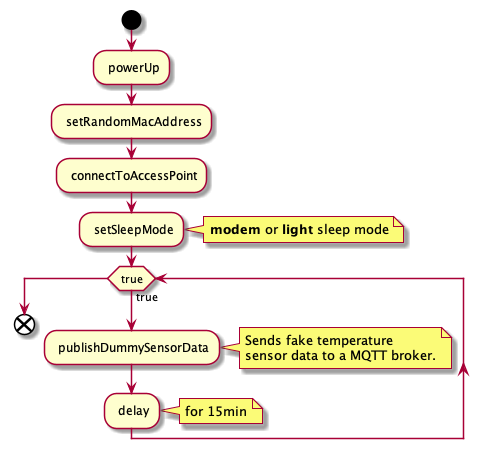
\includegraphics[width = 0.7 \linewidth]{fig/sequence_modem_light_sleep.png}
    \caption{Experimental setup for modem and light sleep.}
    \label{fig:experiment_modem_light_sleep}
\end{figure}

Fig. \ref{fig:experiment_deep_sleep} describes the experimental setup that we used to perform the tests with the deep sleep mode.
After the \textit{enterDeepSleep} step, the ESP8266-01 sleeps for $15min$ and restarts the sequence again.
The difference between deep sleep and modem / light sleep mode is, that the controller restarts the programm everytime it wakes up.\\
TODO: CITE\\
\begin{figure}[H]
    \centering
    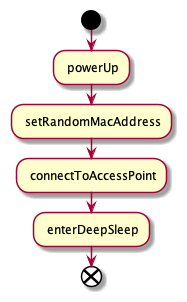
\includegraphics[width = 0.7 \linewidth]{fig/sequence_deep_sleep.png}
    \caption{Experimental setup for deep sleep.}
    \label{fig:experiment_deep_sleep}
\end{figure}

\subsubsection{Modem sleep}
As mentioned in \ref{sec:modem_sleep}, the ESP8266-01 automatically disables the modem when there is no data transmission required.
During transmission the module takes around $80mA$. During modem sleep, $20mA$ are needed.
The modem wakes up every $100ms$ (beacon interval) to keep the connection to the access point established.
Fig. \ref{fig:beacon_interval} shows the beacon interval of $100ms$. 
The same behavior was observed in \cite{montori_is_2017}.

\begin{figure}[H]
    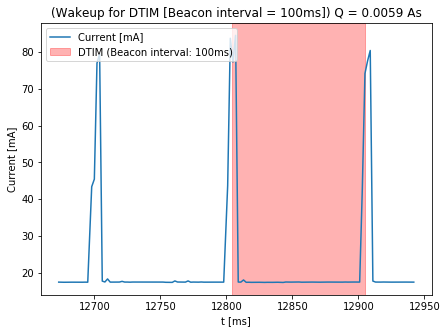
\includegraphics[width = \linewidth]{fig/beacon_interval.png}
    \caption{The power consumption increases to $\approx 80mA$, everytime a beacon arrives.}
    \label{fig:beacon_interval}
\end{figure}

\subsubsection{Light sleep}
As described in \ref{sec:light_sleep}, the light sleep mode disables the CPU when no task has to be processed.
When a task has to be processed, the ESP8266-01 switches back into modem sleep.
Fig. \ref{tab_sleep_modes} shows the change from light sleep (green) to modem sleep (red).
It is clear to see that the ESP8266-01 still needs a lot of power when a beacon arrives (every $100ms$).

\begin{figure}[H]
    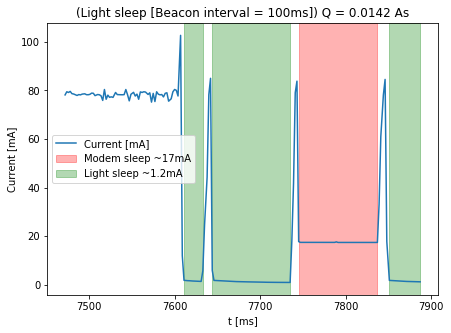
\includegraphics[width = \linewidth]{fig/light_sleep.png}
    \caption{During the light sleep mode, the power consumption of the ESP8266 is drops to 1.2mA.}
    \label{fig:light_sleep}
\end{figure}

\subsubsection{Deep sleep}
The deep sleep mode is the most efficient sleep mode, as described in \ref{sec:deep_sleep}. 
We achieved a power consumption of only $20 \mu A$. 
However, the ESP8266-01 takes a long time to reconnect to the WiFi network after waking up.
Fig. \ref{fig:deep_sleep} shows the power consumtion during the sleep and operating phase.
\begin{figure}[H]
    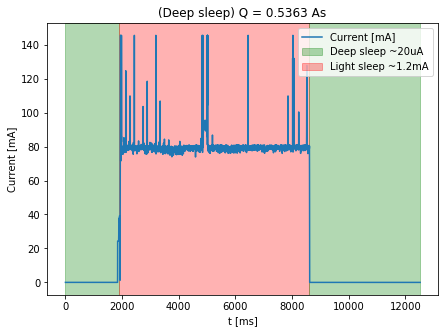
\includegraphics[width = \linewidth]{fig/deep_sleep.png}
    \caption{During deep sleep mode (green), the power consumption drops to $20 \mu A$}
    \label{fig:deep_sleep}
\end{figure}

\section{Results} \label{sec_results}

\section{Conclusions}

\subsection{Some Common Mistakes}\label{SCM}
\begin{itemize}
\item The word ``data'' is plural, not singular.
\item The subscript for the permeability of vacuum $\mu_{0}$, and other common scientific constants, is zero with subscript formatting, not a lowercase letter ``o''.
\item In American English, commas, semicolons, periods, question and exclamation marks are located within quotation marks only when a complete thought or name is cited, such as a title or full quotation. When quotation marks are used, instead of a bold or italic typeface, to highlight a word or phrase, punctuation should appear outside of the quotation marks. A parenthetical phrase or statement at the end of a sentence is punctuated outside of the closing parenthesis (like this). (A parenthetical sentence is punctuated within the parentheses.)
\item A graph within a graph is an ``inset'', not an ``insert''. The word alternatively is preferred to the word ``alternately'' (unless you really mean something that alternates).
\item Do not use the word ``essentially'' to mean ``approximately'' or ``effectively''.
\item In your paper title, if the words ``that uses'' can accurately replace the word ``using'', capitalize the ``u''; if not, keep using lower-cased.
\item Be aware of the different meanings of the homophones ``affect'' and ``effect'', ``complement'' and ``compliment'', ``discreet'' and ``discrete'', ``principal'' and ``principle''.
\item Do not confuse ``imply'' and ``infer''.
\item The prefix ``non'' is not a word; it should be joined to the word it modifies, usually without a hyphen.
\item There is no period after the ``et'' in the Latin abbreviation ``et al.''.
\item The abbreviation ``i.e.'' means ``that is'', and the abbreviation ``e.g.'' means ``for example''.
\end{itemize}
An excellent style manual for science writers is \cite{b7}.

\subsection{Figures and Tables}

\begin{table}[htbp]
\caption{Table Type Styles}
\begin{center}
\begin{tabular}{|c|c|c|c|}
\hline
\textbf{Table}&\multicolumn{3}{|c|}{\textbf{Table Column Head}} \\
\cline{2-4} 
\textbf{Head} & \textbf{\textit{Table column subhead}}& \textbf{\textit{Subhead}}& \textbf{\textit{Subhead}} \\
\hline
copy& More table copy$^{\mathrm{a}}$& &  \\
\hline
\multicolumn{4}{l}{$^{\mathrm{a}}$Sample of a Table footnote.}
\end{tabular}
\label{tab1}
\end{center}
\end{table}

\begin{figure}[htbp]
%\centerline{\includegraphics{fig1.png}}
\caption{Example of a figure caption.}
\label{fig}
\end{figure}

\section*{Acknowledgment}

The preferred spelling of the word ``acknowledgment'' in America is without 
an ``e'' after the ``g''. Avoid the stilted expression ``one of us (R. B. 
G.) thanks $\ldots$''. Instead, try ``R. B. G. thanks$\ldots$''. Put sponsor 
acknowledgments in the unnumbered footnote on the first page.


\printbibliography
\end{document}
